\documentclass[9pt,a4paper,]{extarticle}

\usepackage{f1000_styles}

\usepackage[pdfborder={0 0 0}]{hyperref}

\usepackage[round]{natbib}
\bibliographystyle{unsrtnat}
\let\cite\citep

%% maxwidth is the original width if it is less than linewidth
%% otherwise use linewidth (to make sure the graphics do not exceed the margin)
\makeatletter
\def\maxwidth{ %
  \ifdim\Gin@nat@width>\linewidth
    \linewidth
  \else
    \Gin@nat@width
  \fi
}
\makeatother

\usepackage{color}
\usepackage{fancyvrb}
\newcommand{\VerbBar}{|}
\newcommand{\VERB}{\Verb[commandchars=\\\{\}]}
\DefineVerbatimEnvironment{Highlighting}{Verbatim}{commandchars=\\\{\}}
% Add ',fontsize=\small' for more characters per line
\usepackage{framed}
\definecolor{shadecolor}{RGB}{248,248,248}
\newenvironment{Shaded}{\begin{snugshade}}{\end{snugshade}}
\newcommand{\KeywordTok}[1]{\textcolor[rgb]{0.13,0.29,0.53}{\textbf{#1}}}
\newcommand{\DataTypeTok}[1]{\textcolor[rgb]{0.13,0.29,0.53}{#1}}
\newcommand{\DecValTok}[1]{\textcolor[rgb]{0.00,0.00,0.81}{#1}}
\newcommand{\BaseNTok}[1]{\textcolor[rgb]{0.00,0.00,0.81}{#1}}
\newcommand{\FloatTok}[1]{\textcolor[rgb]{0.00,0.00,0.81}{#1}}
\newcommand{\ConstantTok}[1]{\textcolor[rgb]{0.00,0.00,0.00}{#1}}
\newcommand{\CharTok}[1]{\textcolor[rgb]{0.31,0.60,0.02}{#1}}
\newcommand{\SpecialCharTok}[1]{\textcolor[rgb]{0.00,0.00,0.00}{#1}}
\newcommand{\StringTok}[1]{\textcolor[rgb]{0.31,0.60,0.02}{#1}}
\newcommand{\VerbatimStringTok}[1]{\textcolor[rgb]{0.31,0.60,0.02}{#1}}
\newcommand{\SpecialStringTok}[1]{\textcolor[rgb]{0.31,0.60,0.02}{#1}}
\newcommand{\ImportTok}[1]{#1}
\newcommand{\CommentTok}[1]{\textcolor[rgb]{0.56,0.35,0.01}{\textit{#1}}}
\newcommand{\DocumentationTok}[1]{\textcolor[rgb]{0.56,0.35,0.01}{\textbf{\textit{#1}}}}
\newcommand{\AnnotationTok}[1]{\textcolor[rgb]{0.56,0.35,0.01}{\textbf{\textit{#1}}}}
\newcommand{\CommentVarTok}[1]{\textcolor[rgb]{0.56,0.35,0.01}{\textbf{\textit{#1}}}}
\newcommand{\OtherTok}[1]{\textcolor[rgb]{0.56,0.35,0.01}{#1}}
\newcommand{\FunctionTok}[1]{\textcolor[rgb]{0.00,0.00,0.00}{#1}}
\newcommand{\VariableTok}[1]{\textcolor[rgb]{0.00,0.00,0.00}{#1}}
\newcommand{\ControlFlowTok}[1]{\textcolor[rgb]{0.13,0.29,0.53}{\textbf{#1}}}
\newcommand{\OperatorTok}[1]{\textcolor[rgb]{0.81,0.36,0.00}{\textbf{#1}}}
\newcommand{\BuiltInTok}[1]{#1}
\newcommand{\ExtensionTok}[1]{#1}
\newcommand{\PreprocessorTok}[1]{\textcolor[rgb]{0.56,0.35,0.01}{\textit{#1}}}
\newcommand{\AttributeTok}[1]{\textcolor[rgb]{0.77,0.63,0.00}{#1}}
\newcommand{\RegionMarkerTok}[1]{#1}
\newcommand{\InformationTok}[1]{\textcolor[rgb]{0.56,0.35,0.01}{\textbf{\textit{#1}}}}
\newcommand{\WarningTok}[1]{\textcolor[rgb]{0.56,0.35,0.01}{\textbf{\textit{#1}}}}
\newcommand{\AlertTok}[1]{\textcolor[rgb]{0.94,0.16,0.16}{#1}}
\newcommand{\ErrorTok}[1]{\textcolor[rgb]{0.64,0.00,0.00}{\textbf{#1}}}
\newcommand{\NormalTok}[1]{#1}

% disable code chunks background
%\renewenvironment{Shaded}{}{}

% disable section numbers
\setcounter{secnumdepth}{0}

\setlength{\parindent}{0pt}
\setlength{\parskip}{6pt plus 2pt minus 1pt}



\usepackage{amsthm}
\newtheorem{theorem}{Theorem}
\newtheorem{lemma}{Lemma}
\theoremstyle{definition}
\newtheorem{definition}{Definition}
\newtheorem{corollary}{Corollary}
\newtheorem{proposition}{Proposition}
\theoremstyle{definition}
\newtheorem{example}{Example}
\theoremstyle{definition}
\newtheorem{exercise}{Exercise}
\theoremstyle{remark}
\newtheorem*{remark}{Remark}
\newtheorem*{solution}{Solution}
\begin{document}
\pagestyle{front}

\title{BED: a Biological Entity Dictionary based on a graph data model}

\author[1]{Patrice Godard}
\author[2]{Jonathan van Eyll}
\affil[1]{Corresponding author. Clarivate Analytics, 5901 Priestly Drive, 200, Carlsbad, CA 92008, USA. UCB Pharma, Chemin du Foriest, 1420 Braine-l'Alleud, Belgium patrice.godard@ucb.com.}
\affil[2]{UCB Pharma, Chemin du Foriest, 1420 Braine-l'Alleud, Belgium jonathan.vaneyll@ucb.com.}

\maketitle
\thispagestyle{front}

\begin{abstract}
The understanding of molecular processes involved in a specific biological sytem can be significantly improved by combining and comparing different data set and knowledge resources. However these information sources often use different identification systems and an identifier conversion step is required before any integration effort. Mapping between identifiers is often provided by the reference information resources and several tools have been implemented to simplify their use. However these tools cannot be easily customized and optimized for any specific use. Also the information provided by different resources is not combined to increase the efficiency of the mapping process and deprecated identifiers from former version of databases are not taken into account. Finally finding automatically the most relevant path to map identifiers from one scope to the other is often not trivial. The Biological Entity Dictionary (BED) adresses these challenges by relying on a graph data model describing possible relationships between entities and their identifiers. This model has been implemented using Neo4j and an R package provides functions to query the graph but also to create and feed a custom instance of the database.
\end{abstract}

\section*{Keywords}
genomics, transcriptomics, proteomics, RNA-seq, microarray, database, identifiers.


\clearpage
\pagestyle{main}

\newcommand{\tm}{\textsuperscript{\textregistered}}
\newcommand{\neo}{Neo4j\tm{}}
\newcommand{\cypher}{Cypher\tm{}}
\newcommand{\docker}{Docker\tm{}}
\newcommand{\metabase}{MetaBase\tm{}}

\section{Introduction}\label{introduction}

Since the advent of genome sequencing projects, many technologies have been
developped to get access to different molecular information at a large scale
and with high throughput. DNA microarrays are probably the archetype of such
technology because of their historical impact on gathering data related
to nucleic acids: genomic DNA and RNA. They triggered the emergence of
``omics'' fields of research such as genomics, epigenomics or transcriptomics.
Lately massive parallel sequencing
further increased the throughput of data generation related to nucleic acids
by several orders of magnitude.
In a different way mass spectrometry-related technologies allow the
identification and the quantification of many kinds of molecular entities
such as metabolites and proteins.
Many information systems have been developped to manage
the exploding amount of data and knowledge related to biological
molecular entities.
These resources manage different aspects of
the knowledge.
For example some are genome or proteome centered whereas other
are focused on molecular interactions and pathways.
Thus all these resources rely on different identifier systems to organise
the concepts of interest.
The value of all the experimental data and all the knowledge
collected in public or private resources is very high as such
but is also often synegistically leveraged by their cross comparison
in a dedicated manner. Indeed many datasets can be relevant when
adressing the understanding of a specific biological system, a phenotypic trait
or a disease for example. These datasets can focus on different biological
entities such as transcripts or proteins in different tissues, conditions
or organisms. Comparing all these data and integrating them with
available knowledge require the ability to map the identifiers on which
each resource relies.

To achieve this task public and proprietary information systems
provide mapping tables between their own identifiers and those
from other resources.
Furthermore many tools have been developped to facilitate the access
to this information.
Ensembl BioMarts \citep{kinsella_ensembl_2011},
mygene \citep{wu_biogps_2013},
and g:Profiler \citep{reimand_g:profiler-web_2016}
are popular examples among many others.
However, as pointed by \citet{van_iersel_bridgedb_2010}, these tools
are generally dedicated to a particular domain not necessarly
relevant or complete for all research project and keeping them
up-to-date can also be an issue.
Recognizing these challenges \citet{van_iersel_bridgedb_2010} proposed
the BridgeDb framework providing to bioinformatics developers
a standard interface between tools and
mapping services and also allowing the easy integration of custom data
by a transitivity mechanism.

Here we present BED: a biological entity dictionary.
BED has been developped to adress three main challenges.
The first one is related to the completeness of identifier mappings.
Indeed direct mapping information provided by the different
systems are not always complete and can be enriched by mappings provided
by other resources. More interestingly direct mappings not identified by
any of these resources can be indireclty infered by using mappings to a
third reference. For example many human Ensembl gene identifiers not
directly mapped to any Entrez gene identifiers by neither Ensembl nor the NCBI
can be indirectly mapped using mappings to HGNC identifiers.
The second challenge is related to the mapping of deprecated identifiers.
Indeed entity identifiers can change from one resource release to another.
The identifier history is provided by some resources, such as Ensembl or
the NCBI, but it is generally not used by mapping tools.
The third challenge is related to the automation of the mapping process
according to the relationships between the biological entities of interest.
Indeed mapping between gene and protein identifier scopes should not be done
the same way than two scopes of gene identifiers.
Also converting identifiers from different organism should be possible
using gene ortholog information.

To meet these challenges we designed a graph data model describing possible
relationships between different biological entities and their identifiers.
This data model has been implemented with the \neo{} graph
database \citep{neo4j_inc_neo4j_2017}
and conversion rules have been defined and coded in
an R \citep{r_core_team_r:_2017} package.
We provide an instance of the BED database focused on human, mouse and
rat organism but many functions are available to construct other instances
tailored to other needs.

\section{Methods}\label{methods}

\subsection{Data model}\label{data-model}

\begin{figure}

{\centering 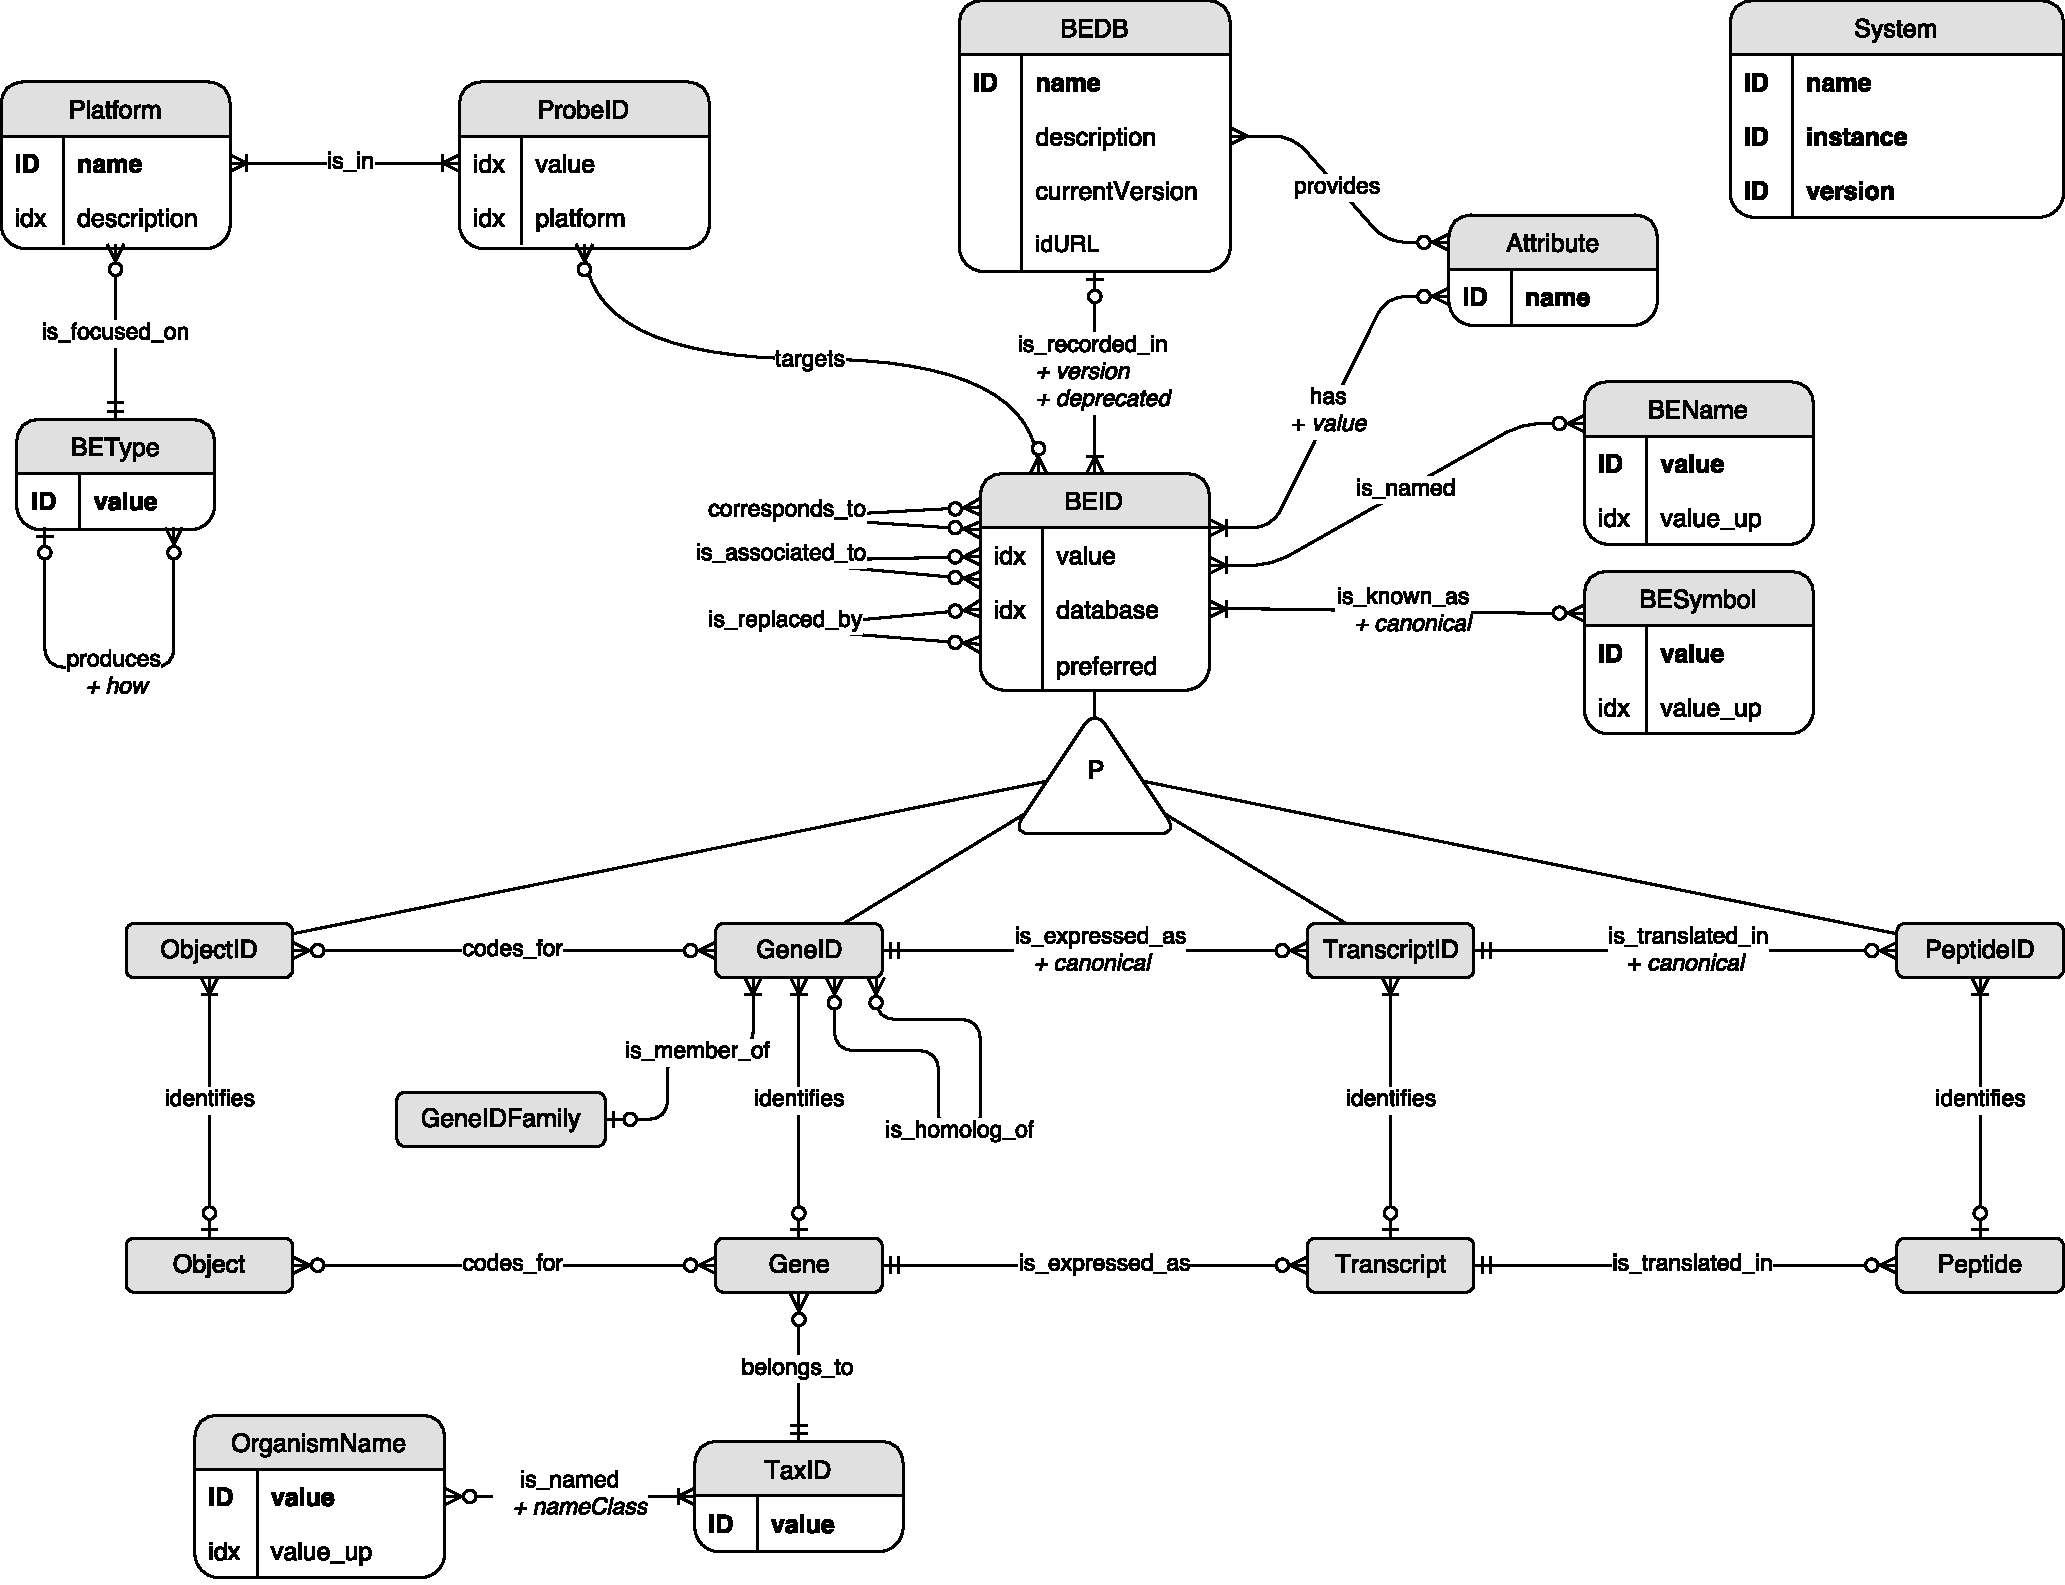
\includegraphics[width=1\linewidth]{img/BED-Data-Model} 

}

\caption{The BED graph data model. The model is shown as an Entity/Relationship (ER) diagram: entities correspond to graph nodes and relationships to graph edges. ``ID'' and ``idx'' indicate if the corresponding entity property is unique or indexed respectively. Some redundancies occur in this data model. Indeed some ``value'' properties are duplicated in upper case (``value\_up'') in order to improve the performance of case-insensitive searches. Also the database of a BEID node is provided as a property to ensure uniqueness of the couples of ``database'' and ``value'' properties. The same approach has been applied for the ``platform'' property of ProbeID nodes.}\label{fig:Data-Model}
\end{figure}

The BED (Biological Entity Dictionary) system relies on a data model
inspired by the central dogma of
molecular biology \citep{crick_central_1970} and describing
relationships between molecular concepts
usually manipulated in the frame of genomics studies
(Figure \ref{fig:Data-Model}).
A biological entity identifier (\emph{BEID}) can identify either a \emph{Gene} (\emph{GeneID}),
a \emph{Transcript} (\emph{TranscriptID}), a \emph{Peptide} (\emph{PeptideID}) or
an \emph{Object} (\emph{ObjectID}). \emph{Object} entities can correspond to complex concepts
coded by any number of genes (i.e.~a protein complex or a molecular function).
\emph{BEID} are extracted from public or private databases (\emph{BEDB}).
\emph{BEDB} can provide an \emph{Attribute} related to each \emph{BEID}.
For example it can be the
sequencing region provided by the Ensembl database \citep{zerbino_ensembl_2017}
or the identifier
status provided by Uniprot \citep{the_uniprot_consortium_uniprot:_2017}.
\emph{BEID} can have one or several associated names (\emph{BENames}) and symbols
(\emph{BESymbol}). \emph{GeneID} can have one or several homologs in other organisms
belonging to the same \emph{GeneIDFamily}.
Many genomics platforms, such as microarray, allow the identification of
biological entity by using probes identified by \emph{ProbeID}. In general
\emph{BEID} can be targeted by several probes belonging to a \emph{Platform} which
is focused on one and only one type of entity (BEType) among those described
above: \emph{Gene}, \emph{Transcript}, \emph{Peptide} or \emph{Object}. A BEType can have several
BEType products but can be the product of at most one BEType.
This constraint allows the unambiguous identification of the most relevant path
to convert identfiers from one scope to another and
is fulfilled by the current data model:
peptides are only produced from transcripts which are only produced
from genes which can also code for objects.

\emph{BEID} identifying the same biological entity are related through three
different kinds of relationship according to the information available
in the source databases and to the decision made by the database administrator
about how to use them. Two \emph{BEID} which \emph{corresponds\_to} each other both
\emph{identify} the same biological entity. A \emph{BEID} which \emph{is\_associated\_to} or
which \emph{is\_replaced\_by} another \emph{BEID} does not directly
identify any biological entity: the link is always indirect through
one or several other \emph{BEID}. Therefore by design a \emph{BEID}
which \emph{is\_associated\_to} or which \emph{is\_replaced\_by} another \emph{BEID} can be
related to several different biological entities. It is not the case for
other \emph{BEID} which identify one and only one biological entity.
This set of possible relationship allows the indirect mapping of
different identifiers not necessarily provided by any integrated resource.

In order to efficiently leverage indirect path through these different
relationships the data model has been implemented in
a \neo{} graph database \citep{neo4j_inc_neo4j_2017}.

\subsection{Feeding the database}\label{feeding-the-database}

Two R \citep{r_core_team_r:_2017} packages have been developed to feed and query
the database.
The first one, neo2R, provides low level functions to interact with
\neo{}. The second R package, BED,
provides functions to feed and query the BED
\neo{} graph database according to the
data model described above.

Many functions are provided within the package to build a tailored BED database
instance. These functions are not exported in order not to mislead
the user when querying the database (which is the expected most frequent
usage of the system). An R markdown document showing how to build a BED database
instance for human, mouse and rat organisms is provided within the
package. It can be adapted to other organisms or needs.

Briefly these functions can be divided according to three main levels:

\begin{itemize}
\item
  The lowest level function is the \texttt{bedImport} function
  which load a table in the \neo{} database according to a \cypher{} query.
\item
  Functions of the second level allow loading identifiers and relationships
  tables ensuring the integrity of the data model.
\item
  Highest level functions are helpers for loading information provided by
  some public resources in different specific format.
\end{itemize}

\subsection{Querying the database}\label{querying-the-database}

The \emph{BED} R package provides several functions to retrieve identifiers
from different resources and also to convert identifiers from one
reference to another.
These functions generate and call \cypher{} queries on the \neo{} database.
Converting thousands of identifiers can take some time
(generally a few seconds). Also such conversions are often recurrent and
redundant. In order to improve the performance for such recurrent and redundant
queries, a cache system has been implemented. The first time, the query is run
on \neo{} for all the relevant ID related to user input and the result is saved
in a local file. Next time similar queries are requested, the system does
not call \neo{} but loads the cached results and filters it according
to user input.
By default the cache is flushed when the system detects inconsistencies
with the BED database. It can also be manually flushed if needed.

\subsection{Operation}\label{operation}

The graph database has been implemented
with \neo{} version 3 \citep{neo4j_inc_neo4j_2017}.
The BED R package depends on the following packages available in the
Comprehensive R Archive Network \citep{cran_comprehensive_nodate}:

\begin{itemize}
\item
  \emph{visNetwork} \citep{almende_b.v._visnetwork:_2017}
\item
  \emph{dplyr} \citep{wickham_dplyr:_2017}
\item
  \emph{htmltools} \citep{rstudio_inc_htmltools:_2017}
\item
  \emph{DT} \citep{xie_dt:_2016}
\item
  \emph{shiny} \citep{chang_shiny:_2017}
\item
  \emph{miniUI} \citep{cheng_miniui:_2016}
\item
  \emph{rstudioapi} \citep{allaire_rstudioapi:_2017}
\end{itemize}

\section{Use Cases}\label{use-cases}

\subsection{Available database instance}\label{available-database-instance}

An instance of the BED database (UCB-Human)
has been built using the script provided
in the BED R package and made available in a \docker{}
image \citep{docker_inc_docker_2017} available here:
\url{https://hub.docker.com/r/patzaw/bed-ucb-human/}

This instance used to exemplify the following use cases
is focused on \emph{Homo sapiens}, \emph{Mus musculus} and \emph{Rattus norvegicus} organisms
and it has been built from the following resources:

\begin{itemize}
\item
  Ensembl \citep{zerbino_ensembl_2017}
\item
  NCBI \citep{ncbi_resource_coordinators_database_2017}
\item
  Uniprot \citep{the_uniprot_consortium_uniprot:_2017}
\item
  biomaRt \citep{durinck_mapping_2009}
\item
  GEOquery \citep{davis_geoquery:_2007}
\item
  Clarivate Analytics \metabase{} \citep{clarivate_analytics_metacore_2017}
\end{itemize}

\begin{table}[htbp]
\caption{\label{tab:ID-Numbers}Numbers of BEID available in the BED UCB-Human database instance.
Numbers have been split according to the BE type
and the organism.
Only BEID which can be mapped to each other are taken into account.}
\centering
\begin{tabledata}{@{}lllrl@{}}
\header BE & Organism & Database & BEID & URL\\
\row Gene & Homo sapiens & MIM\_GENE & 17,146 & \url{http://www.omim.org}\\
\row Gene & Homo sapiens & miRBase & 1,881 & \url{http://www.mirbase.org}\\
\row Gene & Homo sapiens & UniGene & 23,012 & \url{https://www.ncbi.nlm.nih.gov}\\
\row Gene & Homo sapiens & Ens\_gene & 68,460 & \url{http://www.ensembl.org}\\
\row Gene & Homo sapiens & HGNC & 41,195 & \url{http://www.genenames.org}\\
\row Gene & Homo sapiens & EntrezGene & 81,761 & \url{https://www.ncbi.nlm.nih.gov}\\
\row Gene & Homo sapiens & Vega\_gene & 19,141 & \url{http://vega.sanger.ac.uk}\\
\row Gene & Homo sapiens & MetaBase\_gene & 23,377 & \url{https://portal.genego.com}\\
\row Gene & Mus musculus & miRBase & 1,193 & \url{http://www.mirbase.org}\\
\row Gene & Mus musculus & UniGene & 21,576 & \url{https://www.ncbi.nlm.nih.gov}\\
\row Gene & Mus musculus & Ens\_gene & 56,954 & \url{http://www.ensembl.org}\\
\row Gene & Mus musculus & MGI & 78,547 & \url{http://www.informatics.jax.org}\\
\row Gene & Mus musculus & EntrezGene & 103,555 & \url{https://www.ncbi.nlm.nih.gov}\\
\row Gene & Mus musculus & Vega\_gene & 45,237 & \url{http://vega.sanger.ac.uk}\\
\row Gene & Mus musculus & MetaBase\_gene & 20,628 & \url{https://portal.genego.com}\\
\row Gene & Rattus norvegicus & miRBase & 495 & \url{http://www.mirbase.org}\\
\row Gene & Rattus norvegicus & UniGene & 12,613 & \url{https://www.ncbi.nlm.nih.gov}\\
\row Gene & Rattus norvegicus & Ens\_gene & 34,963 & \url{http://www.ensembl.org}\\
\row Gene & Rattus norvegicus & RGD & 46,976 & \url{https://rgd.mcw.edu}\\
\row Gene & Rattus norvegicus & EntrezGene & 57,026 & \url{https://www.ncbi.nlm.nih.gov}\\
\row Gene & Rattus norvegicus & Vega\_gene & 1,146 & \url{http://vega.sanger.ac.uk}\\
\row Gene & Rattus norvegicus & MetaBase\_gene & 17,505 & \url{https://portal.genego.com}\\
\row Transcript & Homo sapiens & Ens\_transcript & 228,389 & \url{http://www.ensembl.org}\\
\row Transcript & Homo sapiens & Vega\_transcript & 37,017 & \url{http://vega.sanger.ac.uk}\\
\row Transcript & Homo sapiens & RefSeq & 189,384 & \url{https://www.ncbi.nlm.nih.gov}\\
\row Transcript & Mus musculus & Ens\_transcript & 136,967 & \url{http://www.ensembl.org}\\
\row Transcript & Mus musculus & Vega\_transcript & 120,271 & \url{http://vega.sanger.ac.uk}\\
\row Transcript & Mus musculus & RefSeq & 112,390 & \url{https://www.ncbi.nlm.nih.gov}\\
\row Transcript & Rattus norvegicus & Ens\_transcript & 42,393 & \url{http://www.ensembl.org}\\
\row Transcript & Rattus norvegicus & Vega\_transcript & 1,271 & \url{http://vega.sanger.ac.uk}\\
\row Transcript & Rattus norvegicus & RefSeq & 98,431 & \url{https://www.ncbi.nlm.nih.gov}\\
\row Peptide & Homo sapiens & Ens\_translation & 109,643 & \url{http://www.ensembl.org}\\
\row Peptide & Homo sapiens & Vega\_translation & 36,460 & \url{http://vega.sanger.ac.uk}\\
\row Peptide & Homo sapiens & RefSeq\_peptide & 117,465 & \url{https://www.ncbi.nlm.nih.gov}\\
\row Peptide & Homo sapiens & Uniprot & 232,130 & \url{http://www.uniprot.org}\\
\row Peptide & Mus musculus & Ens\_translation & 65,406 & \url{http://www.ensembl.org}\\
\row Peptide & Mus musculus & Vega\_translation & 57,318 & \url{http://vega.sanger.ac.uk}\\
\row Peptide & Mus musculus & RefSeq\_peptide & 79,418 & \url{https://www.ncbi.nlm.nih.gov}\\
\row Peptide & Mus musculus & Uniprot & 114,825 & \url{http://www.uniprot.org}\\
\row Peptide & Rattus norvegicus & Ens\_translation & 30,245 & \url{http://www.ensembl.org}\\
\row Peptide & Rattus norvegicus & Vega\_translation & 1,260 & \url{http://vega.sanger.ac.uk}\\
\row Peptide & Rattus norvegicus & RefSeq\_peptide & 68,716 & \url{https://www.ncbi.nlm.nih.gov}\\
\row Peptide & Rattus norvegicus & Uniprot & 40,786 & \url{http://www.uniprot.org}\\
\row Object & Homo sapiens & MetaBase\_object & 24,748 & \url{https://portal.genego.com}\\
\row Object & Homo sapiens & GO\_function & 4,104 & \url{http://amigo.geneontology.org}\\
\row Object & Mus musculus & MetaBase\_object & 22,000 & \url{https://portal.genego.com}\\
\row Object & Mus musculus & GO\_function & 4,081 & \url{http://amigo.geneontology.org}\\
\row Object & Rattus norvegicus & MetaBase\_object & 18,648 & \url{https://portal.genego.com}\\
\row Object & Rattus norvegicus & GO\_function & 4,001 & \url{http://amigo.geneontology.org}\\
\end{tabledata}
\end{table}

The numbers of biological entity (BE) identifiers (BEID) available in this
BED database instance and which can be mapped to each other are shown
in table \ref{tab:ID-Numbers}.
In total, 3,519,181 BEID are available in this
BED instance but many
of them cannot be mapped to other BEID because corresponding to deprecated
identifiers not corresponding to any identifier currently in use.
Also all the genomics platforms included in this BED database instance are
shown in table \ref{tab:Platforms} . They provide mapping to BEID from
354,205 ProbeID in total.

\begin{table}[htbp]
\caption{\label{tab:Platforms}Genomics platforms available in the BED UCB-Human database instance.}
\centering
\begin{tabledata}{@{}lll@{}}
\header Name & Description & BE\\
\row GPL6101 & Illumina ratRef-12 v1.0 expression beadchip & Gene\\
\row GPL6947 & Illumina HumanHT-12 V3.0 expression beadchip & Gene\\
\row GPL10558 & Illumina HumanHT-12 V4.0 expression beadchip & Gene\\
\row GPL1355 & {[}Rat230\_2{]} Affymetrix Rat Genome 230 2.0 Array & Gene\\
\row GPL1261 & {[}Mouse430\_2{]} Affymetrix Mouse Genome 430 2.0 Array & Gene\\
\row GPL96 & {[}HG-U133A{]} Affymetrix Human Genome U133A Array & Gene\\
\row GPL13158 & {[}HT\_HG-U133\_Plus\_PM{]} Affymetrix HT HG-U133+ PM Array Plate & Gene\\
\row GPL571 & {[}HG-U133A\_2{]} Affymetrix Human Genome U133A 2.0 Array & Gene\\
\row GPL570 & {[}HG-U133\_Plus\_2{]} Affymetrix Human Genome U133 Plus 2.0 Array & Gene\\
\row GPL6480 & Agilent-014850 Whole Human Genome Microarray 4x44K G4112F & Gene\\
\row GPL6885 & Illumina MouseRef-8 v2.0 expression beadchip & Transcript\\
\end{tabledata}
\end{table}

\subsection{Exploring identifiers of biological entities}\label{exploring-identifiers-of-biological-entities}

The \texttt{getBeIds} function returns all BE identifiers from a specific scope.
A scopes is defined
by the type of BE or probe, the source of the identifiers (database or platform)
and the organism.
For example the following code
returns all the Ensembl identifiers of human genes.

\begin{Shaded}
\begin{Highlighting}[]
\NormalTok{beids <-}\StringTok{ }\KeywordTok{getBeIds}\NormalTok{(}
    \DataTypeTok{be=}\StringTok{"Gene"}\NormalTok{, }\DataTypeTok{source=}\StringTok{"Ens_gene"}\NormalTok{, }\DataTypeTok{organism=}\StringTok{"human"}\NormalTok{,}
    \DataTypeTok{restricted=}\OtherTok{FALSE}
\NormalTok{)}
\KeywordTok{head}\NormalTok{(beids)}
\end{Highlighting}
\end{Shaded}

\begin{verbatim}
##                    id preferred  Gene db.version db.deprecated
## 82643 ENSG00000283891      TRUE 64781         91         FALSE
## 82642 ENSG00000207766      TRUE 64783         91         FALSE
## 82645 ENSG00000276678      TRUE 64785         91         FALSE
## 82644 ENSG00000265993      TRUE 64787         91         FALSE
## 82647 ENSG00000283793      TRUE 64789         91         FALSE
## 82646 ENSG00000283621      TRUE 64791         91         FALSE
\end{verbatim}

\begin{figure}

{\centering 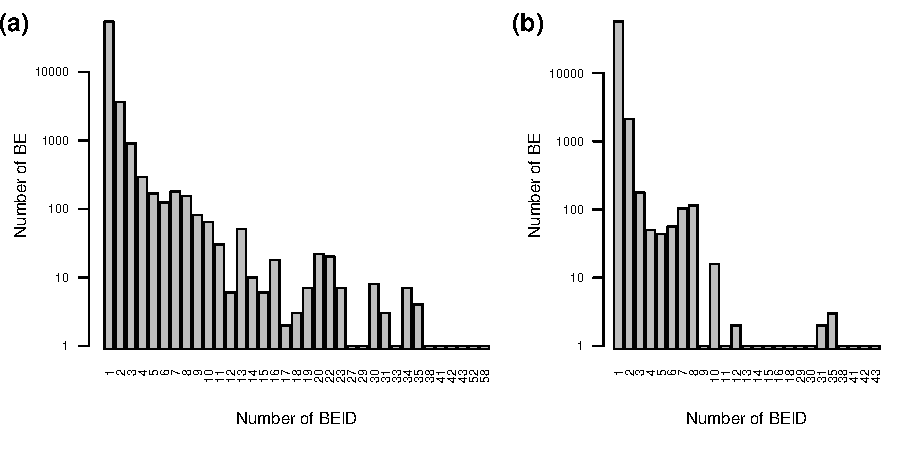
\includegraphics[width=1\linewidth]{BED-F1000-Article_files/figure-latex/beidTables-1} 

}

\caption{Barplots showing the number of gene BE (log scale) identified by one or more Ensembl gene BEID. a) All Ensembl gene BEID. b) Current Ensembl gene ID (version 91).}\label{fig:beidTables}
\end{figure}

The \emph{id} column corresponds to the BEID from the source of interest.
The column named according to the BE type (in this case \emph{Gene})
corresponds to the internal identifiers of the related BE.
This internal identifier is not a stable reference that can be used as such.
Nevertheless it is useful to identify BEID identifying the
same BE.
In the example above even if most of Gene BE are identified by only
one Ensembl gene BEID, many of them are identified by two or more
(5,809
/ 59,515
= 10~\%);
277 BE
are even identified by more than 10 Ensembl BEID
(Figure \ref{fig:beidTables}.a).
In this case, most of these redundancies come from deprecated ID from former
versions of the Ensembl database (version in used here: 91)
and can be excluded by setting the \texttt{restricted} parameter to \texttt{TRUE} when calling
the \texttt{getBeIds} function (Figure \ref{fig:beidTables}.b).
However many BE are still identified by two or more current Ensembl BEID
(2,715
/ 59,515
= 5\textasciitilde{}\%).
This result comes from the way the BED database is constructed:
When two identifiers from the same resource correspond to the same identifier
in another resource (\emph{correspond\_to} relationship in the data model),
all these BEID are considered to identify the same BE.

A complex example of such mapping is shown in figure \ref{fig:TAS2R8}
mapping all the BEID of the human TAS2R8 gene which codes for a protein
of the family of candidate taste receptors. There are three identifiers
corresponding to this gene symbol in Ensembl. All these three identifiers
correspond to the same Entrez gene and the same HGNC identifiers.
All these BEID are thus considered to identify the same gene. It turns out
that the three Ensembl BEID correspond to the same gene mapped on different
sequence version of the chromosome 12: the canonical (ENSG00000121314),
CHR\_HSCHR12\_2\_CTG2 (ENSG00000272712)
and CHR\_HSCHR12\_3\_CTG2 (ENSG00000277316).
This information provided by Ensembl is encoded in the \emph{seq\_region}
attribute for each Ensembl BEID (see data model)
and is used to define \emph{preferred} BEID which are mapped on canonical version
of chromosome sequences.
The ENSG00000272712 identifier shows also a complex history in former
Ensembl versions.

\begin{figure}

{\centering 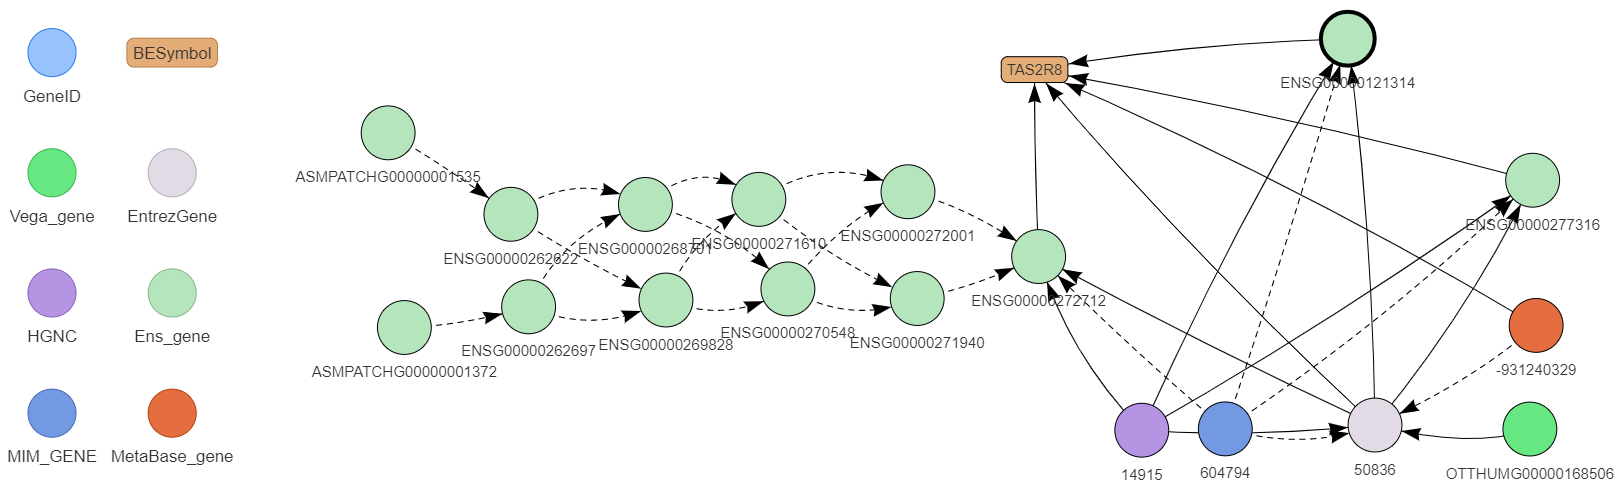
\includegraphics[width=1\linewidth]{img/TAS2R8-Identifiers} 

}

\caption{BED relationshsips between all the different identifiers of the human TAS2R8 gene recorded in the database. BEID are shown as circle and gene symbol in the rounded box. The color legend is shown to the left of the figure. BEID surrounded in bold correspond to \emph{preferred} identifiers. Solid arrows represent \emph{correspond\_to} and \emph{is\_known\_as} relationships. Dotted arrows represent \emph{is\_replaced\_by} and \emph{is\_associated\_to} relationships. This graph has been drawn with the \texttt{exploreBe} function.}\label{fig:TAS2R8}
\end{figure}

\subsection{Converting identifiers}\label{converting-identifiers}

The main goal of BED is to convert identifiers from one scope to another
easily, rapidly and with high completeness.
It has been thought in order to allow recurring comparisons to each other of
many lists of biological entities from various origins.

The function \texttt{guessIdOrigin} can be used to guess the scope
of any list of identifiers.
A simple example regarding the conversion of human Ensembl
gene to human Entrez gene identifiers is shown below and discussed hereafter.
By setting the \texttt{restricted} parameter to \texttt{TRUE} the converted BEID are
restricted to current - non-deprecated - version of Entrez gene identifiers.
Nevertheless all the input BEID are taken into account,
current and deprecated ones.

\begin{Shaded}
\begin{Highlighting}[]
\NormalTok{bedConv <-}\StringTok{ }\KeywordTok{convBeIds}\NormalTok{(}
   \DataTypeTok{ids=}\NormalTok{beids}\OperatorTok{$}\NormalTok{id, }\DataTypeTok{from=}\StringTok{"Gene"}\NormalTok{, }\DataTypeTok{from.source=}\StringTok{"Ens_gene"}\NormalTok{, }\DataTypeTok{from.org=}\StringTok{"human"}\NormalTok{,}
   \DataTypeTok{to.source=}\StringTok{"EntrezGene"}\NormalTok{, }\DataTypeTok{restricted=}\OtherTok{TRUE}
\NormalTok{)}
\end{Highlighting}
\end{Shaded}

Among all the 68,460
human Ensembl gene identifiers available in the
database, 21,718
(32~\%)
were not converted to any human Entrez gene
identifier: 21,073
(33~\%)
of the 64,661 non-deprecated
and 645
(17~\%)
of the 3,799 deprecated identifiers.

Three other tools were used on Jan 04, 2018
to perform the same conversion task:
biomaRt \citep{kinsella_ensembl_2011, durinck_mapping_2009},
mygene \citep{wu_biogps_2013, mark_mygene:_2014},
and gProfileR \citep{reimand_g:profiler-web_2016, reimand_gprofiler:_2016}.
At that time, biomaRt and mygene were based on the Ensembl 91 release
whereas gProfileR was based on release 90.

\begin{figure}

{\centering 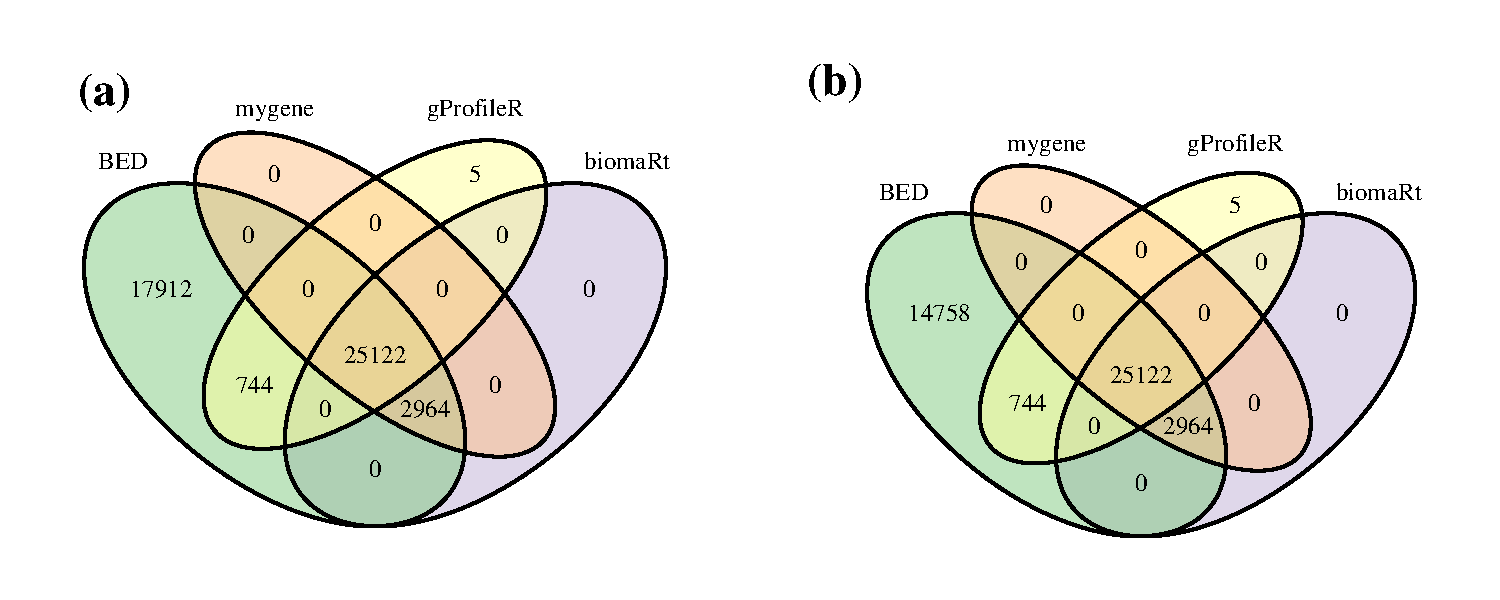
\includegraphics[width=1\linewidth]{BED-F1000-Article_files/figure-latex/vennTools-1} 

}

\caption{Venn diagrams showing the number of human Ensembl gene identifiers mapped to at least one human Entrez gene identifier by the different tested tools when focusing (a) on all 68,460 or (b) on current 64,661 BEID (Ensembl 91 release).}\label{fig:vennTools}
\end{figure}

The numbers of human Ensembl gene identifiers successfully converted by each
method are compared in figure \ref{fig:vennTools}.
Five identifiers were only converted by gProfileR.
They were provided by former versions of Ensembl or NCBI
but are now deprecated in the current releases of these two resources.
All the other gene identifiers converted by the different methods
were also converted by BED. However BED was able to map at least
17,912 more identifiers than all the
other tools (figure \ref{fig:vennTools}.a). A few of these mappings
(3,154)
are explained by the fact that BED is the only tool mapping
deprecated identifiers to current versions.
Nevertheless, even when focusing on the mapping of current versions of
Ensembl identifiers BED was able to
map 14,758
more identifiers than all the
other tools (figure \ref{fig:vennTools}.b).
A few of these mappings (627)
are directly provided by the NCBI. But most of them
(14,131)
are inferred from a mapping of the Ensembl and Entrez gene identifiers
to the same HGNC \citep{gray_genenames.org:_2015} identifier.

A rough approximation of running times of the different methods is provided
in table \ref{tab:runTimes}. The aim of this table is to show that BED,
as a dedicated and localy available tool,
is a very efficient option to convert large lists of identifiers on the fly and
recurrently.
The aim of BED is to improve the efficiency of identifier conversion
in a well defined context (organism, information resources of interest\ldots{})
and not to replace biomaRt, mygene, gProfileR
or other tools which provide many more features
for many organisms and which should not be narrowed to this task for a
complete comparison.

\begin{table}[htbp]
\caption{\label{tab:runTimes}Rough approximation of running time of different methods
to convert human Ensembl gene identifiers in human Entrez gene identifiers.}
\centering
\begin{tabledata}{@{}ll@{}}
\header Method & Running time\\
\row BED (Not cached) & \textasciitilde{}9.9 secs\\
\row BED (Cached) & \textasciitilde{}2.5 secs\\
\row biomaRt & \textasciitilde{}40 secs\\
\row mygene & \textasciitilde{}3.9 mins\\
\row gProfileR & \textasciitilde{}1.2 mins\\
\end{tabledata}
\end{table}

The BED \texttt{convBeIds} function can be used to convert identifiers from
any available scope to any other one. It automaticaly find the most
relevant path according to the considered biological entities.
It allows elaborate mapping such as the conversion between
probe identifiers from a platform focused on mouse transcripts into
human protein identifiers.
Because such mappings can be intricated,
BED also provides a function to show the shortest relevant path between
two different identifiers (Figure \ref{fig:explConv}).

\begin{figure}

{\centering 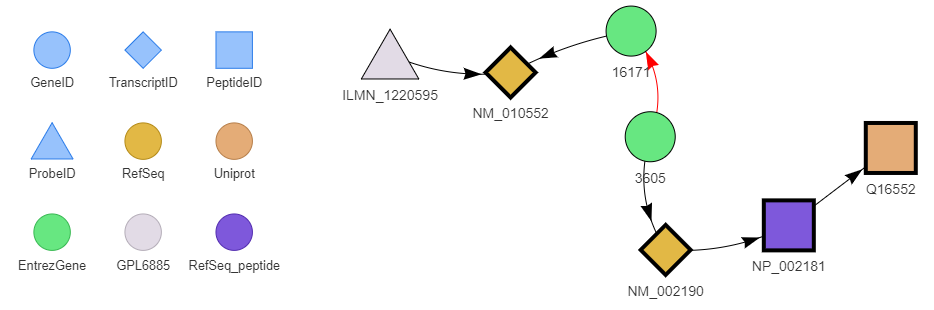
\includegraphics[width=1\linewidth]{img/ILMN_1220595-Conversion} 

}

\caption{BED conversion shortest path between the ILMN\_1220595 probe identifier targeting a transcript of the mouse Il17a gene and the Uniprot Q16552 identifier of the human IL17 protein. The legend is shown to the left of the figure. The red arrow represents the \emph{is\_homolog\_of} relationship. This graph has been drawn with the \texttt{exploreConvPath} function.}\label{fig:explConv}
\end{figure}

\subsection{Additional features}\label{additional-features}

Some additional use cases and examples are provided in
the BED R package vignette.
Several functions are available for annotating BEID with symbols and names,
again taking advantage of information related to connected identifiers.
Other functions are also provided to seek relevant identifier of a specific
biological entity. These functions are used by a shiny \citep{chang_shiny:_2017}
gadget (Figure \ref{fig:findBe})
providing an interactive dictionary of BEID which is also made
available as an Rstudio addin \citep{cheng_miniui:_2016, allaire_rstudioapi:_2017}.

\begin{figure}

{\centering 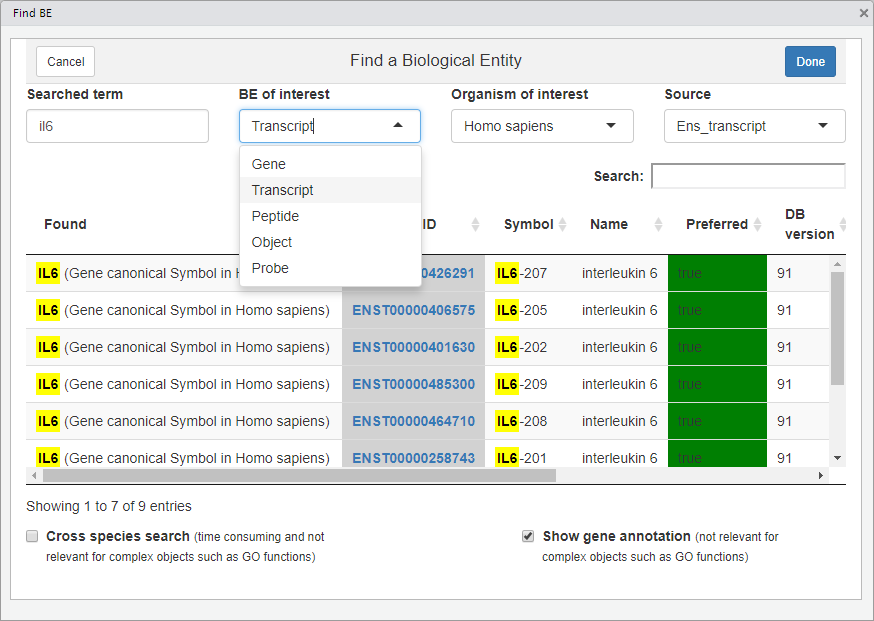
\includegraphics[width=0.8\linewidth]{img/findBe} 

}

\caption{\texttt{findBe} Shiny gadget to seek relevant identifier of a specific biological entity. In this example the user is looking after human Ensembl transcript identifiers corresponding to ``il6''.}\label{fig:findBe}
\end{figure}

\section{Summary}\label{summary}

BED is a system dedicated to the mapping between identifiers of molecular
biological entities. It relies on a graph data model implemented with
\neo{} and on rules coded in an R package.
BED leverages mapping information provided by different resources in order
to increase the mapping efficiency between each of them.
It also allows the mapping of deprecated identifiers.
Rules are used to automatically convert identifiers from one scope to another
using the most appropriate path.

The intend of BED is to be tailored to specific needs and
beside functions for querying the system the BED R package provides functions
to build custom instances of the database.
Database instances can be localy installed or shared accross a community.
This design combined with a cache system makes BED performant for converting
large lists of identifiers from and to a large variety of scopes.

Because of our research field we provide an instance focused on human,
mouse and rat organisms. This database instance can be directly used
in relevant projects but it can also be enriched depending on user or
community needs.

\section{Software availability}\label{software-availability}

This section will be generated by the Editorial Office before publication. Authors are asked to provide some initial information to assist the Editorial Office, as detailed below.

\begin{enumerate}
\def\labelenumi{\arabic{enumi}.}
\item
  URL link to where the software can be downloaded from or used by a non-coder (AUTHOR TO PROVIDE; optional): NO
\item
  URL link to the author's version control system repository containing the source code (AUTHOR TO PROVIDE; required):
\end{enumerate}

\begin{itemize}
\item
  \url{https://github.com/patzaw/BED}
\item
  \url{https://github.com/patzaw/neo2R}
\end{itemize}

\begin{enumerate}
\def\labelenumi{\arabic{enumi}.}
\setcounter{enumi}{2}
\item
  Link to source code as at time of publication (\emph{F1000Research} TO GENERATE)
\item
  Link to archived source code as at time of publication (\emph{F1000Research} TO GENERATE)
\item
  Software license (AUTHOR TO PROVIDE; required): GPL-3
\end{enumerate}

\section{Author contributions}\label{author-contributions}

PG designed and implemented the BED graph database,
the neo2R and BED R packages.
PG and JVE defined use cases, tested the whole system and
wrote the manuscript.

\section{Competing interests}\label{competing-interests}

No competing interests were disclosed.

\section{Grant information}\label{grant-information}

This work was entirely supported by UCB Pharma.
The authors declared that no grants were involved in supporting this work.

\section{Acknowledgments}\label{acknowledgments}

We are grateful to Frédéric Vanclef, Malte Lucken, Liesbeth François,
Matthew Page,
Massimo de Francesco, and Marina Bessarabova for fruitful discussions
and constructive criticisms.

{\small\bibliography{BED-References.bib}}

\end{document}
